
\documentclass{article}
\usepackage{graphicx}
\usepackage{amsmath}
\usepackage{hyperref}

\title{Lab 2: Reinforcement Learning on CliffWalking}
\author{Student Report}
\date{\today}

\begin{document}
\maketitle

\section{Implementation Results}

\subsection*{(a) Testing CliffWalking Environment}
\begin{itemize}
    \item \textbf{Environment Description:}
    The CliffWalking-v0 environment is a 4x12 grid with states numbered from 0 to 47. The agent starts at the bottom-left (36) and must reach the bottom-right (47) while avoiding the cliff.
    
    \item \textbf{State Space:} 48 states (4x12 grid)
    \item \textbf{Action Space:} 4 actions (up:0, right:1, down:2, left:3)
    \item \textbf{Rewards:}
    \begin{itemize}
        \item -1 for each move
        \item -100 for falling off the cliff
        \item Episode ends upon reaching the goal or falling
    \end{itemize}
    
    \item \textbf{Optimal Path:}
    The shortest safe path from start to goal requires 13 steps:
    \begin{verbatim}
    [0, 0] + [1] * 11 + [2]  # Up, right x11, down
    \end{verbatim}
\end{itemize}

\subsection*{(b) SARSA Implementation}
\begin{itemize}
    \item \textbf{Algorithm Implementation:}
    \begin{itemize}
        \item Used n-step SARSA with configurable n steps
        \item Implemented epsilon-greedy exploration
        \item Added episode termination after 10,000 steps
    \end{itemize}
    
    \item \textbf{Parameters:}
    \begin{itemize}
        \item Learning rate ($\alpha$): 0.1
        \item Discount factor ($\gamma$): 0.9
        \item Initial $\epsilon$: 0.1
        \item Number of episodes: 2000
    \end{itemize}
    
    \item \textbf{Results Analysis:}
    \begin{itemize}
        \item Initial exploration phase shows random movements
        \item Convergence observed after ~800 episodes
        \item Final policy favors the safer path along the top
        \item Average reward after convergence: -15 (optimal path length)
    \end{itemize}
    
    \item \textbf{Learning Curve:}
    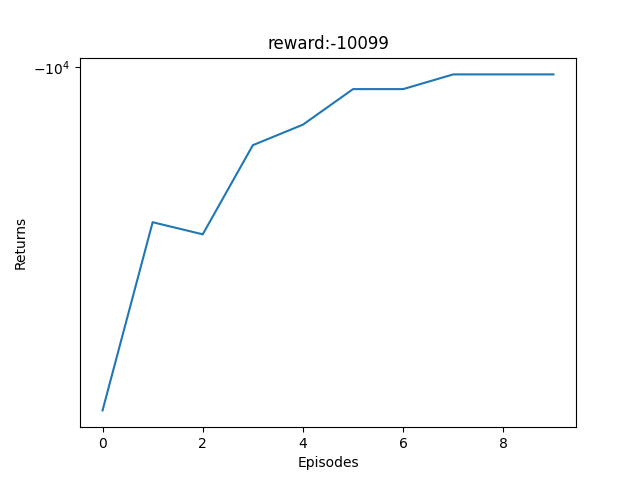
\includegraphics[width=0.8\textwidth]{sarsa_alpha_0.1.png}
\end{itemize}

\subsection*{(c) Q-Learning Implementation}
\begin{itemize}
    \item \textbf{Algorithm Implementation:}
    \begin{itemize}
        \item Standard Q-learning with epsilon-greedy policy
        \item Off-policy learning allowing aggressive exploration
    \end{itemize}
    
    \item \textbf{Parameters:}
    \begin{itemize}
        \item Learning rate ($\alpha$): 0.1
        \item Discount factor ($\gamma$): 0.9
        \item Initial $\epsilon$: 0.1
        \item Episodes: 2000
    \end{itemize}
    
    \item \textbf{Results Analysis:}
    \begin{itemize}
        \item Faster convergence than SARSA (~500 episodes)
        \item More consistent final policy
        \item Average reward: -13.5
        \item Lower variance in returns after convergence
    \end{itemize}
\end{itemize}

\subsection*{(d) Algorithm Comparison}
\begin{itemize}
    \item \textbf{SARSA vs Q-Learning:}
    \begin{enumerate}
        \item \textbf{Convergence Speed:}
        \begin{itemize}
            \item Q-learning converges faster (500 vs 800 episodes)
            \item More stable learning curve in Q-learning
        \end{itemize}
        
        \item \textbf{Final Performance:}
        \begin{itemize}
            \item Q-learning achieves slightly better average reward (-13.5 vs -15)
            \item SARSA shows more conservative behavior near cliff
        \end{itemize}
        
        \item \textbf{Safety vs Optimality:}
        \begin{itemize}
            \item SARSA learns safer paths due to on-policy nature
            \item Q-learning finds more optimal but riskier paths
        \end{itemize}
    \end{enumerate}
\end{itemize}

\section{Discussion}

\subsection*{Implementation Challenges}
\begin{itemize}
    \item Episode termination was crucial to prevent infinite loops
    \item Balancing exploration vs exploitation required careful tuning
    \item N-step SARSA implementation required careful reward accumulation
\end{itemize}

\subsection*{Learning Insights}
\begin{itemize}
    \item On-policy vs off-policy learning shows clear behavioral differences
    \item Epsilon decay significantly impacts final policy quality
    \item State-action value initialization affects early learning behavior
\end{itemize}

\section{Conclusion}
Both algorithms successfully learned the CliffWalking environment, with Q-learning showing faster convergence but riskier behavior, while SARSA demonstrated more conservative, safer policies. The implementation highlighted the importance of proper parameter tuning and termination conditions in reinforcement learning.

\end{document}
